% Môn: Vật lý
% Lớp: 12
% Chương: Chương II. Khí lí tưởng
% Bài: L12C2 Bài 8. Mô hình động học phân tử chất khí · Phân biệt đặc điểm cấu trúc phân tử của chất ở thể rắn, lỏng, khí
% ID: L12C1B1-TN-42
% Mức: NB
% ID: L12C1B1-91-TN


% ID: L12C1B1-TN-4
% Mức: NB
% ID: L12C1B1-97-TN
% ID: L12C1B1-97-TN
% Mức: NB
% ID: L12C1B1-97-TN
% Mức: NB
% ID: L12C1B1-97-TN
% ID: L12C1B1-97-TN
% Mức: NB
% ID: L12C2B8-61-TN
%=== Câu 7 ===%
\dangbt{Phân biệt đặc điểm cấu trúc phân tử của chất ở thể rắn, lỏng, khí}
\begin{ex}
% ID: L12C2B8-61-TN
% Mức: NB
	{\color{red}\footnotesize\ttfamily [L12C1B1-TN-4]}\par %HienID
	Chất rắn có hình dạng nhất định vì các phân tử trong chất rắn
	\choice
	{\True được liên kết chặt chẽ và có trật tự}
	{có thể di chuyển tự do}
	{bị hút về phía trung tâm bởi lực hấp dẫn mạnh}
	{được sắp xếp ngẫu nhiên và rời rạc}
	\loigiai{Các phân tử trong thể rắn có thứ tự sắp xếp trật tự chặc chẽ, lực tương tác mạnh, không cho di chuyển tự do, chỉ có thể dao động quanh vị trí cân bằng xác định}
\end{ex}

% ID: L12C1B1-TN-6
% Mức: NB
% ID: L12C1B1-98-TN
% ID: L12C1B1-98-TN
% Mức: NB
% ID: L12C1B1-98-TN
% Mức: NB
% ID: L12C1B1-98-TN
% ID: L12C1B1-98-TN
% Mức: NB
% ID: L12C2B8-62-TN
%=== Câu 8 ===%
\begin{ex}
% ID: L12C2B8-62-TN
% Mức: NB
	{\color{red}\footnotesize\ttfamily [L12C1B1-TN-6]}\par %HienID
	Đặc điểm nào sau đây là đúng với cấu trúc của chất ở thể lỏng?
	\choice
	{Các phân tử có lực tương tác rất yếu}
	{Các phân tử chuyển động hỗn loạn và có khoảng cách rất lớn}
	{Giữa các phân tử không có khoảng cách}
	{\True Các phân tử dao động quanh vị trí cân bằng, vị trí cân bằng có thể dịch chuyển}
	\loigiai{Các chất ở thể lỏng có các phân tử dao động quanh vị trí cân bằng, vị trí cân bằng có thể dịch chuyển.}
\end{ex}

% ID: L12C1B1-TN-9
% Mức: TH
% ID: L12C1B1-99-TN
% ID: L12C1B1-99-TN
% Mức: TH
% ID: L12C1B1-99-TN
% Mức: TH
% ID: L12C1B1-99-TN
% ID: L12C1B1-99-TN
% Mức: TH
% ID: L12C2B8-63-TN
%=== Câu 9 ===%
\begin{ex}
% ID: L12C2B8-63-TN
% Mức: TH
	{\color{red}\footnotesize\ttfamily [L12C1B1-TN-9]}\par %HienID
	Hình vẽ dưới đây mô tả, so sánh khoảng cách và sự sắp xếp các phân tử ở các thể khác nhau (a), chuyển động của phân tử ở các thể khác nhau (b). Hình nào mô tả cấu trúc của thể rắn?
	\begin{center}
		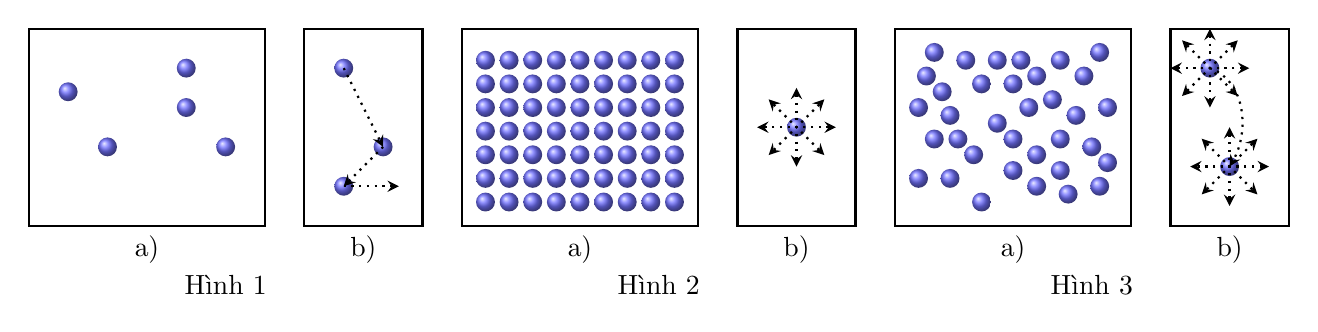
\begin{tikzpicture}[>=stealth, thick]
			
			\draw (0,0) rectangle (3,2.5)
			(3.5,0) rectangle (5,2.5);
			
			\foreach \x/\y in {1/1, 0.5/1.7, 2/2, 2/1.5, 2.5/1} {
				\shade[ball color=blue!60, opacity=0.95] (\x,\y) circle (0.12cm);
			}
			
			\foreach \x/\y in {4/2, 4.5/1, 4/0.5} {
				\shade[ball color=blue!60, opacity=0.95] (\x,\y) circle (0.12cm);
			}
			
			\node[below] at (1.5,0) {a)};
			\node[below] at (4.25,0) {b)};
			\node[below] at (2.5,-0.5) {Hình 1};
			
			\draw[->, dotted] (4,2) -- (4.5,1);
			\draw[->, dotted] (4.5,1) -- (4,0.5);
			\draw[->, dotted] (4,0.5) -- (4.7,0.5);
			
			\begin{scope}[shift={(5.5,0)}]
				\draw (0,0) rectangle (3,2.5)
				(3.5,0) rectangle (5,2.5);
				
				\node[below] at (1.5,0) {a)};
				\node[below] at (4.25,0) {b)};
				\node[below] at (2.5,-0.5) {Hình 2};
				
				\foreach \x in {0.3,0.6,...,3.0}{
					\foreach \y in {0.3,0.6,...,2.4}{
						\shade[ball color=blue!60, opacity=0.95] (\x,\y) circle(0.12cm);
					}
				}
				
				\shade[ball color=blue!60, opacity=0.95] (4.25,1.25) circle(0.12cm);
				
				\foreach \x/\y in {0/180,45/-135,90/-90,135/-45}{
					\draw[<->, dotted]
					({4.25+0.5*cos(\x)},{1.25+0.5*sin(\x)})
					-- ({4.25+0.5*cos(\y)},{1.25+0.5*sin(\y)});
				}
			\end{scope}
			
			\begin{scope}[shift={(11,0)}]
				\draw (0,0) rectangle (3,2.5)
				(3.5,0) rectangle (5,2.5);
				
				\node[below] at (1.5,0) {a)};
				\node[below] at (4.25,0) {b)};
				\node[below] at (2.5,-0.5) {Hình 3};
				
				\foreach \x/\y in {
					0.7/0.6, 1.5/1.1, 1.8/1.9, 1.5/0.7, 2.5/1.0,
					1.1/1.8, 0.8/1.1, 1.1/0.3, 2.1/1.1, 0.5/1.1,
					0.7/1.4, 2.6/0.5, 2.7/1.5, 1.3/1.3, 0.9/2.1,
					1.5/1.8, 1.8/0.5, 2.4/1.9, 0.3/0.6, 0.4/1.9,
					1.0/0.9, 2.0/1.6, 1.3/2.1, 1.7/1.5, 2.6/2.2,
					2.1/2.1, 2.2/0.4, 2.1/0.7, 1.8/0.9, 2.3/1.4,
					0.3/1.5, 0.6/1.7, 1.6/2.1, 2.7/0.8, 0.5/2.2
				}{
					\shade[ball color=blue!60, opacity=0.95] (\x,\y) circle(0.12cm);
				}
				
				\shade[ball color=blue!60, opacity=0.95] (4,2) circle(0.12cm);
				\shade[ball color=blue!60, opacity=0.95] (4.25,0.75) circle(0.12cm);
				
				\foreach \x/\y in {0/180,45/-135,90/-90,135/-45}{
					\draw[<->, dotted] 
					({4+0.5*cos(\x)},{2+0.5*sin(\x)}) -- ({4+0.5*cos(\y)},{2+0.5*sin(\y)});
					\draw[<->, dotted] 
					({4.25+0.5*cos(\x)},{0.75+0.5*sin(\x)}) -- ({4.25+0.5*cos(\y)},{0.75+0.5*sin(\y)});
				}
				
				\draw[->, dotted] (4,2) [out=-20,in=60] to (4.25,0.75);
				
			\end{scope}
			
		\end{tikzpicture}
		
	\end{center}
	\choice
	{\True Hình $(2)$}
	{Hình $(1)$}
	{Hình $(3)$}
	{Hình $(2)$ và $(3)$}
	\loigiai{Các phân tử trong thể rắn có thứ tự sắp xếp trật tự chặc chẽ, lực tương tác mạnh, không cho di chuyển tự do, chỉ có thể dao động quanh vị trí cân bằng xác định}
\end{ex}

% ID: L12C1B1-DS-15
% Mức: TH
% ID: L12C1B1-138-DS
% ID: L12C1B1-138-DS
% Mức: TH
% ID: L12C1B1-138-DS
% Mức: TH
% ID: L12C1B1-138-DS
% ID: L12C1B1-138-DS
% Mức: TH
% ID: L12C2B8-64-DS
%=== Câu 51 ===%
\begin{ex}
% ID: L12C2B8-64-DS
% Mức: TH
	{\color{red}\footnotesize\ttfamily [L12C1B1-DS-15]}\par %HienID
	Xét cấu trúc phân tử của chất ở ba thể rắn, lỏng, khí.
	\choiceTF
	{\True Trong chất rắn, các phân tử dao động quanh các vị trí cân bằng cố định}
	{Trong chất khí, khoảng cách trung bình giữa các phân tử nhỏ hơn nhiều so với trong chất rắn}
	{\True Chất lỏng có thể tích xác định vì các phân tử ở khá gần nhau, nhưng không có hình dạng xác định vì vị trí cân bằng của các phân tử có thể dịch chuyển}
	{Chất khí có thể bị nén dễ dàng vì các phân tử khí liên kết với nhau rất chặt chẽ}
	\loigiai{
		\begin{itemchoice}
			\item Trong chất rắn, lực liên kết phân tử rất mạnh nên các phân tử chỉ có thể dao động quanh các vị trí cân bằng cố định trong mạng tinh thể (hoặc mạng vô định hình). Mệnh đề đúng.
			\item Trong chất khí, khoảng cách trung bình giữa các phân tử lớn hơn rất nhiều so với trong chất rắn (gấp hàng chục lần), không phải nhỏ hơn. Mệnh đề sai.
			\item Ở thể lỏng, các phân tử ở khá gần nhau nên giữ được một thể tích xác định; tuy nhiên vị trí cân bằng của chúng có thể dịch chuyển được nên chất lỏng không có hình dạng riêng. Mệnh đề đúng.
			\item Chất khí dễ bị nén không phải vì các phân tử liên kết chặt chẽ, mà ngược lại là do lực liên kết giữa các phân tử khí rất yếu và khoảng cách giữa chúng rất lớn (còn nhiều khoảng trống), nên dễ dàng bị ép lại gần nhau hơn. Mệnh đề sai.
		\end{itemchoice}
	}
\end{ex}

% ID: L12C1B1-DS-16
% Mức: TH
% ID: L12C1B1-139-DS
% ID: L12C1B1-139-DS
% Mức: TH
% ID: L12C1B1-139-DS
% Mức: TH
% ID: L12C1B1-139-DS
% ID: L12C1B1-139-DS
% Mức: TH
% ID: L12C2B8-65-DS
%=== Câu 52 ===%
\begin{ex}
% ID: L12C2B8-65-DS
% Mức: TH
	{\color{red}\footnotesize\ttfamily [L12C1B1-DS-16]}\par %HienID
	Xét sự so sánh cấu trúc phân tử giữa ba thể rắn, lỏng, khí.
	\choiceTF
	{\True Thứ tự sắp xếp có trật tự nhất đến kém trật tự nhất của các phân tử là: rắn, lỏng, khí}
	{Khoảng cách trung bình giữa các phân tử ở thể lỏng lớn hơn ở thể khí}
	{Lực liên kết phân tử ở thể khí là mạnh nhất trong ba thể}
	{\True Chất khí không có hình dạng riêng vì các phân tử chuyển động hỗn loạn, không bị giữ ở vị trí cố định}
	\loigiai{
		\begin{itemchoice}
			\item Ở thể rắn, các phân tử sắp xếp có trật tự chặt chẽ nhất; ở thể lỏng, trật tự sắp xếp kém hơn nhưng vẫn còn khá gần nhau; ở thể khí, các phân tử phân bố hỗn loạn, hầu như không có trật tự. Mệnh đề đúng.
			\item Ngược lại, khoảng cách trung bình giữa các phân tử ở thể khí lớn hơn rất nhiều so với ở thể lỏng, không phải nhỏ hơn. Mệnh đề sai.
			\item Lực liên kết phân tử ở thể khí là yếu nhất trong ba thể (do khoảng cách phân tử rất lớn), không phải mạnh nhất. Mệnh đề sai.
			\item Ở thể khí, các phân tử chuyển động hỗn loạn tự do theo mọi hướng và không bị giữ ở vị trí cố định nào, nên khối khí luôn lan tỏa để chiếm toàn bộ thể tích bình chứa mà không có hình dạng riêng. Mệnh đề đúng.
		\end{itemchoice}
	}
\end{ex}

% ID: L12C1B1-TLN-3
% Mức: TH
% ID: L12C1B1-151-TLN
% ID: L12C1B1-151-TLN
% Mức: TH
% ID: L12C1B1-151-TLN
% Mức: TH
% ID: L12C1B1-151-TLN
% ID: L12C1B1-151-TLN
% Mức: TH
% ID: L12C2B8-66-TLN
%=== Câu 64 ===%
\begin{bt}
% ID: L12C2B8-66-TLN
% Mức: TH
	{\color{red}\footnotesize\ttfamily [L12C1B1-TLN-3]}\par %HienID
	Cho các phát biểu sau về cấu trúc phân tử của các thể:\\
	(1) Ở thể rắn, các phân tử dao động quanh vị trí cân bằng cố định.\\
	(2) Ở thể lỏng, các phân tử dao động quanh vị trí cân bằng có thể dịch chuyển.\\
	(3) Ở thể khí, khoảng cách giữa các phân tử rất nhỏ.\\
	(4) Chất khí luôn chiếm toàn bộ thể tích bình chứa.\\
	Có bao nhiêu phát biểu đúng?
	\shortans[oly]{$3$}
	\loigiai{
		Phát biểu (1), (2), (4) đúng. Phát biểu (3) sai vì ở thể khí, khoảng cách giữa các phân tử rất lớn (không phải rất nhỏ). Vậy có $3$ phát biểu đúng.
	}
\end{bt}

% ID: L12C1B1-TLN-4
% Mức: TH
% ID: L12C1B1-152-TLN
% ID: L12C1B1-152-TLN
% Mức: TH
% ID: L12C1B1-152-TLN
% Mức: TH
% ID: L12C1B1-152-TLN
% ID: L12C1B1-152-TLN
% Mức: TH
% ID: L12C2B8-67-TLN
%=== Câu 65 ===%
\begin{bt}
% ID: L12C2B8-67-TLN
% Mức: TH
	{\color{red}\footnotesize\ttfamily [L12C1B1-TLN-4]}\par %HienID
	Cho các phát biểu sau:\\
	(1) Chất rắn có thể tích và hình dạng riêng xác định.\\
	(2) Chất lỏng có thể tích riêng nhưng không có hình dạng riêng.\\
	(3) Chất khí không có thể tích và hình dạng riêng.\\
	(4) Chất rắn dễ bị nén hơn chất khí.\\
	Có bao nhiêu phát biểu đúng?
	\shortans[oly]{$3$}
	\loigiai{
		Phát biểu (1), (2), (3) đúng. Phát biểu (4) sai vì chất khí dễ bị nén hơn chất rắn rất nhiều (do khoảng cách phân tử khí lớn hơn nhiều). Vậy có $3$ phát biểu đúng.
	}
\end{bt}

% ID: L12C1B1-TL-2
% Mức: VD
% ID: L12C1B1-161-TL
% ID: L12C1B1-161-TL
% Mức: VD
% ID: L12C1B1-161-TL
% Mức: VD
% ID: L12C1B1-161-TL
% ID: L12C1B1-161-TL
% Mức: VD
% ID: L12C2B8-68-TL
%=== Câu 74 ===%
\begin{bt}
% ID: L12C2B8-68-TL
% Mức: VD
	{\color{red}\footnotesize\ttfamily [L12C1B1-TL-2]}\par %HienID
	\begin{enumerate}
		\item Nêu điểm khác biệt về khoảng cách phân tử, lực liên kết và kiểu chuyển động của phân tử ở ba thể rắn, lỏng, khí.
		\item Dựa vào ý 1), giải thích tại sao có thể nén khí dễ dàng nhưng rất khó nén chất lỏng hoặc chất rắn.
		\item Giải thích tại sao một lượng khí luôn chiếm toàn bộ thể tích của bình chứa nó, trong khi một lượng chất lỏng chỉ chiếm một phần thể tích của bình chứa (nếu bình có thể tích lớn hơn thể tích chất lỏng).
	\end{enumerate}
	\loigiai{
		\begin{enumerate}
			\item Ở thể rắn: khoảng cách giữa các phân tử rất nhỏ, lực liên kết rất mạnh, các phân tử chỉ dao động quanh vị trí cân bằng cố định. Ở thể lỏng: khoảng cách giữa các phân tử nhỏ (xấp xỉ thể rắn), lực liên kết tương đối mạnh nhưng yếu hơn ở thể rắn, các phân tử dao động quanh vị trí cân bằng có thể dịch chuyển. Ở thể khí: khoảng cách giữa các phân tử rất lớn, lực liên kết rất yếu (gần như không đáng kể), các phân tử chuyển động hỗn loạn tự do theo mọi hướng.
			\item Ở thể khí, do khoảng cách giữa các phân tử rất lớn nên còn nhiều "khoảng trống" giữa chúng; khi bị nén, các phân tử dễ dàng xích lại gần nhau hơn. Ở thể lỏng và thể rắn, các phân tử đã ở rất gần nhau nên lực đẩy giữa chúng tăng rất nhanh khi khoảng cách giảm thêm, khiến chúng rất khó bị nén.
			\item Ở thể khí, các phân tử chuyển động hỗn loạn tự do và lực liên kết giữa chúng gần như không đáng kể, nên chúng lan tỏa ra mọi hướng cho đến khi chiếm toàn bộ thể tích bình chứa. Ở thể lỏng, lực liên kết phân tử đủ mạnh để giữ các phân tử ở gần nhau tạo thành một thể tích xác định, nên chất lỏng chỉ chiếm phần thể tích tương ứng với lượng chất lỏng đó, không lan tỏa ra chiếm toàn bộ bình chứa.
		\end{enumerate}
	}
\end{bt}

% ===== Câu 89 =====
% ID: L12C2B8-69-DS
% Mức: NB
\begin{ex}
% ID: L12C2B8-69-DS
% Mức: NB
Xét các phát biểu sau về dạng “Phân biệt đặc điểm cấu trúc phân tử của chất ở thể rắn, lỏng, khí” (bộ số 4).
\choiceTF
{\True Khoảng cách phân tử trung bình tăng theo thứ tự rắn, lỏng, khí.}
{Các phân tử chất khí chỉ dao động quanh vị trí cân bằng cố định.}
{\True Khi giải dạng “Phân biệt đặc điểm cấu trúc phân tử của chất ở thể rắn, lỏng, khí”, cần xác định đúng trạng thái đầu, trạng thái cuối và quy ước dấu hoặc điều kiện áp dụng.}
{Có thể bỏ qua mọi dữ kiện về khối lượng, nhiệt độ và hiệu suất trong mọi bài toán thuộc dạng này.}
\loigiai{
\begin{itemchoice}
\item (Đúng) Khoảng cách phân tử trung bình tăng theo thứ tự rắn, lỏng, khí. (Vì): Khoảng cách phân tử trung bình tăng theo thứ tự rắn, lỏng, khí. b) S: Các phân tử chất khí chỉ dao động quanh vị trí cân bằng cố định. c) Đ: Khi giải dạng “Phân biệt đặc điểm cấu trúc phân tử của chất ở thể rắn, lỏng, khí”, cần xác định đúng trạng thái đầu, trạng thái cuối và quy ước dấu hoặc điều kiện áp dụng. d) S: Có thể bỏ qua mọi dữ kiện về khối lượng, nhiệt độ và hiệu suất trong mọi bài toán thuộc dạng này. Kết luận dựa trên định nghĩa, điều kiện áp dụng và quy ước trong SGK KNTT
\item (Sai) Các phân tử chất khí chỉ dao động quanh vị trí cân bằng cố định.
\item (Đúng) Khi giải dạng “Phân biệt đặc điểm cấu trúc phân tử của chất ở thể rắn, lỏng, khí”, cần xác định đúng trạng thái đầu, trạng thái cuối và quy ước dấu hoặc điều kiện áp dụng.
\item (Sai) Có thể bỏ qua mọi dữ kiện về khối lượng, nhiệt độ và hiệu suất trong mọi bài toán thuộc dạng này.
\end{itemchoice}
}
\end{ex}

% ===== Câu 93 =====
% ID: L12C2B8-70-DS
% Mức: TH
\begin{ex}
% ID: L12C2B8-70-DS
% Mức: TH
Xét các phát biểu sau về dạng “Phân biệt đặc điểm cấu trúc phân tử của chất ở thể rắn, lỏng, khí” (bộ số 1).
\choiceTF
{Các phân tử chất khí chỉ dao động quanh vị trí cân bằng cố định.}
{\True Khi giải dạng “Phân biệt đặc điểm cấu trúc phân tử của chất ở thể rắn, lỏng, khí”, cần xác định đúng trạng thái đầu, trạng thái cuối và quy ước dấu hoặc điều kiện áp dụng.}
{Có thể bỏ qua mọi dữ kiện về khối lượng, nhiệt độ và hiệu suất trong mọi bài toán thuộc dạng này.}
{\True Khoảng cách phân tử trung bình tăng theo thứ tự rắn, lỏng, khí.}
\loigiai{
\begin{itemchoice}
\item (Sai) Các phân tử chất khí chỉ dao động quanh vị trí cân bằng cố định. (Vì): Các phân tử chất khí chỉ dao động quanh vị trí cân bằng cố định. b) Đ: Khi giải dạng “Phân biệt đặc điểm cấu trúc phân tử của chất ở thể rắn, lỏng, khí”, cần xác định đúng trạng thái đầu, trạng thái cuối và quy ước dấu hoặc điều kiện áp dụng. c) S: Có thể bỏ qua mọi dữ kiện về khối lượng, nhiệt độ và hiệu suất trong mọi bài toán thuộc dạng này. d) Đ: Khoảng cách phân tử trung bình tăng theo thứ tự rắn, lỏng, khí. Kết luận dựa trên định nghĩa, điều kiện áp dụng và quy ước trong SGK KNTT
\item (Đúng) Khi giải dạng “Phân biệt đặc điểm cấu trúc phân tử của chất ở thể rắn, lỏng, khí”, cần xác định đúng trạng thái đầu, trạng thái cuối và quy ước dấu hoặc điều kiện áp dụng.
\item (Sai) Có thể bỏ qua mọi dữ kiện về khối lượng, nhiệt độ và hiệu suất trong mọi bài toán thuộc dạng này.
\item (Đúng) Khoảng cách phân tử trung bình tăng theo thứ tự rắn, lỏng, khí.
\end{itemchoice}
}
\end{ex}

% ===== Câu 97 =====
% ID: L12C2B8-71-DS
% Mức: TH
\begin{ex}
% ID: L12C2B8-71-DS
% Mức: TH
Xét các phát biểu sau về dạng “Phân biệt đặc điểm cấu trúc phân tử của chất ở thể rắn, lỏng, khí” (bộ số 5).
\choiceTF
{Các phân tử chất khí chỉ dao động quanh vị trí cân bằng cố định.}
{\True Khi giải dạng “Phân biệt đặc điểm cấu trúc phân tử của chất ở thể rắn, lỏng, khí”, cần xác định đúng trạng thái đầu, trạng thái cuối và quy ước dấu hoặc điều kiện áp dụng.}
{Có thể bỏ qua mọi dữ kiện về khối lượng, nhiệt độ và hiệu suất trong mọi bài toán thuộc dạng này.}
{\True Khoảng cách phân tử trung bình tăng theo thứ tự rắn, lỏng, khí.}
\loigiai{
\begin{itemchoice}
\item (Sai) Các phân tử chất khí chỉ dao động quanh vị trí cân bằng cố định. (Vì): Các phân tử chất khí chỉ dao động quanh vị trí cân bằng cố định. b) Đ: Khi giải dạng “Phân biệt đặc điểm cấu trúc phân tử của chất ở thể rắn, lỏng, khí”, cần xác định đúng trạng thái đầu, trạng thái cuối và quy ước dấu hoặc điều kiện áp dụng. c) S: Có thể bỏ qua mọi dữ kiện về khối lượng, nhiệt độ và hiệu suất trong mọi bài toán thuộc dạng này. d) Đ: Khoảng cách phân tử trung bình tăng theo thứ tự rắn, lỏng, khí. Kết luận dựa trên định nghĩa, điều kiện áp dụng và quy ước trong SGK KNTT
\item (Đúng) Khi giải dạng “Phân biệt đặc điểm cấu trúc phân tử của chất ở thể rắn, lỏng, khí”, cần xác định đúng trạng thái đầu, trạng thái cuối và quy ước dấu hoặc điều kiện áp dụng.
\item (Sai) Có thể bỏ qua mọi dữ kiện về khối lượng, nhiệt độ và hiệu suất trong mọi bài toán thuộc dạng này.
\item (Đúng) Khoảng cách phân tử trung bình tăng theo thứ tự rắn, lỏng, khí.
\end{itemchoice}
}
\end{ex}

% ===== Câu 98 =====
% ID: L12C2B8-72-TL
% Mức: NB
\begin{bt}
% ID: L12C2B8-72-TL
% Mức: NB
Trình bày cách nhận biết và phương pháp giải dạng “Phân biệt đặc điểm cấu trúc phân tử của chất ở thể rắn, lỏng, khí”. Phân tích nhận định sau và sửa lại nếu sai: “Các phân tử chất khí chỉ dao động quanh vị trí cân bằng cố định.”
\loigiai{
Trước hết xác định hiện tượng, trạng thái và các đại lượng đã cho. Nêu định nghĩa hoặc hệ thức phù hợp, đổi về đơn vị SI, áp dụng đúng điều kiện và kiểm tra ý nghĩa kết quả. Nhận định cần đối chiếu: Khoảng cách phân tử trung bình tăng theo thứ tự rắn, lỏng, khí. Vì vậy nhận định đã cho sai; phát biểu đúng là: Khoảng cách phân tử trung bình tăng theo thứ tự rắn, lỏng, khí.
}
\end{bt}

% ===== Câu 99 =====
% ID: L12C2B8-73-TLN
% Mức: NB
\begin{ex}
% ID: L12C2B8-73-TLN
% Mức: NB
Cho bốn nhận định: (1) Khoảng cách phân tử trung bình tăng theo thứ tự rắn, lỏng, khí. (2) Các phân tử chất khí chỉ dao động quanh vị trí cân bằng cố định. (3) Cần kiểm tra đơn vị và điều kiện áp dụng khi xử lí dạng “Phân biệt đặc điểm cấu trúc phân tử của chất ở thể rắn, lỏng, khí”. (4) Có thể thay tùy ý nhiệt độ Celsius cho nhiệt độ tuyệt đối trong mọi công thức. Có bao nhiêu nhận định đúng? Trả lời bằng một số nguyên.
\shortans{2}
\loigiai{
Nhận định (1) và (3) đúng; (2) và (4) sai. Vậy có 2 nhận định đúng.
}
\end{ex}

% ===== Câu 101 =====
% ID: L12C2B8-74-DS
% Mức: VD
\begin{ex}
% ID: L12C2B8-74-DS
% Mức: VD
Xét các phát biểu sau về dạng “Phân biệt đặc điểm cấu trúc phân tử của chất ở thể rắn, lỏng, khí” (bộ số 2).
\choiceTF
{\True Khi giải dạng “Phân biệt đặc điểm cấu trúc phân tử của chất ở thể rắn, lỏng, khí”, cần xác định đúng trạng thái đầu, trạng thái cuối và quy ước dấu hoặc điều kiện áp dụng.}
{Có thể bỏ qua mọi dữ kiện về khối lượng, nhiệt độ và hiệu suất trong mọi bài toán thuộc dạng này.}
{\True Khoảng cách phân tử trung bình tăng theo thứ tự rắn, lỏng, khí.}
{Các phân tử chất khí chỉ dao động quanh vị trí cân bằng cố định.}
\loigiai{
\begin{itemchoice}
\item (Đúng) Khi giải dạng “Phân biệt đặc điểm cấu trúc phân tử của chất ở thể rắn, lỏng, khí”, cần xác định đúng trạng thái đầu, trạng thái cuối và quy ước dấu hoặc điều kiện áp dụng. (Vì): Khi giải dạng “Phân biệt đặc điểm cấu trúc phân tử của chất ở thể rắn, lỏng, khí”, cần xác định đúng trạng thái đầu, trạng thái cuối và quy ước dấu hoặc điều kiện áp dụng. b) S: Có thể bỏ qua mọi dữ kiện về khối lượng, nhiệt độ và hiệu suất trong mọi bài toán thuộc dạng này. c) Đ: Khoảng cách phân tử trung bình tăng theo thứ tự rắn, lỏng, khí. d) S: Các phân tử chất khí chỉ dao động quanh vị trí cân bằng cố định. Kết luận dựa trên định nghĩa, điều kiện áp dụng và quy ước trong SGK KNTT
\item (Sai) Có thể bỏ qua mọi dữ kiện về khối lượng, nhiệt độ và hiệu suất trong mọi bài toán thuộc dạng này.
\item (Đúng) Khoảng cách phân tử trung bình tăng theo thứ tự rắn, lỏng, khí.
\item (Sai) Các phân tử chất khí chỉ dao động quanh vị trí cân bằng cố định.
\end{itemchoice}
}
\end{ex}

% ===== Câu 104 =====
% ID: L12C1B1-26-TN
% Mức: NB

% ===== Câu 105 =====
% ID: L12C2B8-75-DS
% Mức: VDC
\begin{ex}
% ID: L12C2B8-75-DS
% Mức: VDC
Xét các phát biểu sau về dạng “Phân biệt đặc điểm cấu trúc phân tử của chất ở thể rắn, lỏng, khí” (bộ số 3).
\choiceTF
{Có thể bỏ qua mọi dữ kiện về khối lượng, nhiệt độ và hiệu suất trong mọi bài toán thuộc dạng này.}
{\True Khoảng cách phân tử trung bình tăng theo thứ tự rắn, lỏng, khí.}
{Các phân tử chất khí chỉ dao động quanh vị trí cân bằng cố định.}
{\True Khi giải dạng “Phân biệt đặc điểm cấu trúc phân tử của chất ở thể rắn, lỏng, khí”, cần xác định đúng trạng thái đầu, trạng thái cuối và quy ước dấu hoặc điều kiện áp dụng.}
\loigiai{
\begin{itemchoice}
\item (Sai) Có thể bỏ qua mọi dữ kiện về khối lượng, nhiệt độ và hiệu suất trong mọi bài toán thuộc dạng này. (Vì): Có thể bỏ qua mọi dữ kiện về khối lượng, nhiệt độ và hiệu suất trong mọi bài toán thuộc dạng này. b) Đ: Khoảng cách phân tử trung bình tăng theo thứ tự rắn, lỏng, khí. c) S: Các phân tử chất khí chỉ dao động quanh vị trí cân bằng cố định. d) Đ: Khi giải dạng “Phân biệt đặc điểm cấu trúc phân tử của chất ở thể rắn, lỏng, khí”, cần xác định đúng trạng thái đầu, trạng thái cuối và quy ước dấu hoặc điều kiện áp dụng. Kết luận dựa trên định nghĩa, điều kiện áp dụng và quy ước trong SGK KNTT
\item (Đúng) Khoảng cách phân tử trung bình tăng theo thứ tự rắn, lỏng, khí.
\item (Sai) Các phân tử chất khí chỉ dao động quanh vị trí cân bằng cố định.
\item (Đúng) Khi giải dạng “Phân biệt đặc điểm cấu trúc phân tử của chất ở thể rắn, lỏng, khí”, cần xác định đúng trạng thái đầu, trạng thái cuối và quy ước dấu hoặc điều kiện áp dụng.
\end{itemchoice}
}
\end{ex}

% ===== Câu 106 =====
% ID: L12C2B8-76-TL
% Mức: TH
\begin{bt}
% ID: L12C2B8-76-TL
% Mức: TH
Trình bày cách nhận biết và phương pháp giải dạng “Phân biệt đặc điểm cấu trúc phân tử của chất ở thể rắn, lỏng, khí”. Phân tích nhận định sau và sửa lại nếu sai: “Khoảng cách phân tử trung bình tăng theo thứ tự rắn, lỏng, khí.”
\loigiai{
Trước hết xác định hiện tượng, trạng thái và các đại lượng đã cho. Nêu định nghĩa hoặc hệ thức phù hợp, đổi về đơn vị SI, áp dụng đúng điều kiện và kiểm tra ý nghĩa kết quả. Nhận định cần đối chiếu: Khoảng cách phân tử trung bình tăng theo thứ tự rắn, lỏng, khí. Vì vậy nhận định đã cho đúng.
}
\end{bt}

% ===== Câu 175 =====
% ID: L12C2B8-77-TN
% Mức: NB
\begin{ex}
% ID: L12C2B8-77-TN
% Mức: NB
Câu 1 thuộc dạng “Phân biệt đặc điểm cấu trúc phân tử của chất ở thể rắn, lỏng, khí”. Phát biểu nào sau đây đúng?
\choice
{Các phân tử chất khí chỉ dao động quanh vị trí cân bằng cố định.}
{Nhiệt lượng và nhiệt độ là hai đại lượng hoàn toàn giống nhau.}
{Mọi quá trình nhiệt học đều không phụ thuộc điều kiện thực hiện.}
{\True Khoảng cách phân tử trung bình tăng theo thứ tự rắn, lỏng, khí.}
\loigiai{
Phát biểu đúng là: Khoảng cách phân tử trung bình tăng theo thứ tự rắn, lỏng, khí. Các phương án còn lại trái với mô hình, định nghĩa hoặc hệ thức nhiệt học tương ứng.
}
\end{ex}

% ===== Câu 176 =====
% ID: L12C2B8-78-TN
% Mức: NB
\begin{ex}
% ID: L12C2B8-78-TN
% Mức: NB
Câu 5 thuộc dạng “Phân biệt đặc điểm cấu trúc phân tử của chất ở thể rắn, lỏng, khí”. Phát biểu nào sau đây đúng?
\choice
{Các phân tử chất khí chỉ dao động quanh vị trí cân bằng cố định.}
{Nhiệt lượng và nhiệt độ là hai đại lượng hoàn toàn giống nhau.}
{Mọi quá trình nhiệt học đều không phụ thuộc điều kiện thực hiện.}
{\True Khoảng cách phân tử trung bình tăng theo thứ tự rắn, lỏng, khí.}
\loigiai{
Phát biểu đúng là: Khoảng cách phân tử trung bình tăng theo thứ tự rắn, lỏng, khí. Các phương án còn lại trái với mô hình, định nghĩa hoặc hệ thức nhiệt học tương ứng.
}
\end{ex}

% ===== Câu 177 =====
% ID: L12C2B8-79-TN
% Mức: NB
\begin{ex}
% ID: L12C2B8-79-TN
% Mức: NB
Câu 9 thuộc dạng “Phân biệt đặc điểm cấu trúc phân tử của chất ở thể rắn, lỏng, khí”. Phát biểu nào sau đây đúng?
\choice
{Các phân tử chất khí chỉ dao động quanh vị trí cân bằng cố định.}
{Nhiệt lượng và nhiệt độ là hai đại lượng hoàn toàn giống nhau.}
{Mọi quá trình nhiệt học đều không phụ thuộc điều kiện thực hiện.}
{\True Khoảng cách phân tử trung bình tăng theo thứ tự rắn, lỏng, khí.}
\loigiai{
Phát biểu đúng là: Khoảng cách phân tử trung bình tăng theo thứ tự rắn, lỏng, khí. Các phương án còn lại trái với mô hình, định nghĩa hoặc hệ thức nhiệt học tương ứng.
}
\end{ex}

% ===== Câu 178 =====
% ID: L12C2B8-80-TN
% Mức: TH
\begin{ex}
% ID: L12C2B8-80-TN
% Mức: TH
Câu 2 thuộc dạng “Phân biệt đặc điểm cấu trúc phân tử của chất ở thể rắn, lỏng, khí”. Phát biểu nào sau đây đúng?
\choice
{Nhiệt lượng và nhiệt độ là hai đại lượng hoàn toàn giống nhau.}
{Mọi quá trình nhiệt học đều không phụ thuộc điều kiện thực hiện.}
{\True Khoảng cách phân tử trung bình tăng theo thứ tự rắn, lỏng, khí.}
{Các phân tử chất khí chỉ dao động quanh vị trí cân bằng cố định.}
\loigiai{
Phát biểu đúng là: Khoảng cách phân tử trung bình tăng theo thứ tự rắn, lỏng, khí. Các phương án còn lại trái với mô hình, định nghĩa hoặc hệ thức nhiệt học tương ứng.
}
\end{ex}

% ===== Câu 179 =====
% ID: L12C2B8-81-TN
% Mức: TH
\begin{ex}
% ID: L12C2B8-81-TN
% Mức: TH
Câu 6 thuộc dạng “Phân biệt đặc điểm cấu trúc phân tử của chất ở thể rắn, lỏng, khí”. Phát biểu nào sau đây đúng?
\choice
{Nhiệt lượng và nhiệt độ là hai đại lượng hoàn toàn giống nhau.}
{Mọi quá trình nhiệt học đều không phụ thuộc điều kiện thực hiện.}
{\True Khoảng cách phân tử trung bình tăng theo thứ tự rắn, lỏng, khí.}
{Các phân tử chất khí chỉ dao động quanh vị trí cân bằng cố định.}
\loigiai{
Phát biểu đúng là: Khoảng cách phân tử trung bình tăng theo thứ tự rắn, lỏng, khí. Các phương án còn lại trái với mô hình, định nghĩa hoặc hệ thức nhiệt học tương ứng.
}
\end{ex}

% ===== Câu 180 =====
% ID: L12C2B8-82-TN
% Mức: TH
\begin{ex}
% ID: L12C2B8-82-TN
% Mức: TH
Câu 10 thuộc dạng “Phân biệt đặc điểm cấu trúc phân tử của chất ở thể rắn, lỏng, khí”. Phát biểu nào sau đây đúng?
\choice
{Nhiệt lượng và nhiệt độ là hai đại lượng hoàn toàn giống nhau.}
{Mọi quá trình nhiệt học đều không phụ thuộc điều kiện thực hiện.}
{\True Khoảng cách phân tử trung bình tăng theo thứ tự rắn, lỏng, khí.}
{Các phân tử chất khí chỉ dao động quanh vị trí cân bằng cố định.}
\loigiai{
Phát biểu đúng là: Khoảng cách phân tử trung bình tăng theo thứ tự rắn, lỏng, khí. Các phương án còn lại trái với mô hình, định nghĩa hoặc hệ thức nhiệt học tương ứng.
}
\end{ex}

% ===== Câu 181 =====
% ID: L12C2B8-83-TN
% Mức: VD
\begin{ex}
% ID: L12C2B8-83-TN
% Mức: VD
Câu 3 thuộc dạng “Phân biệt đặc điểm cấu trúc phân tử của chất ở thể rắn, lỏng, khí”. Phát biểu nào sau đây đúng?
\choice
{Mọi quá trình nhiệt học đều không phụ thuộc điều kiện thực hiện.}
{\True Khoảng cách phân tử trung bình tăng theo thứ tự rắn, lỏng, khí.}
{Các phân tử chất khí chỉ dao động quanh vị trí cân bằng cố định.}
{Nhiệt lượng và nhiệt độ là hai đại lượng hoàn toàn giống nhau.}
\loigiai{
Phát biểu đúng là: Khoảng cách phân tử trung bình tăng theo thứ tự rắn, lỏng, khí. Các phương án còn lại trái với mô hình, định nghĩa hoặc hệ thức nhiệt học tương ứng.
}
\end{ex}

% ===== Câu 182 =====
% ID: L12C2B8-84-TN
% Mức: VD
\begin{ex}
% ID: L12C2B8-84-TN
% Mức: VD
Câu 7 thuộc dạng “Phân biệt đặc điểm cấu trúc phân tử của chất ở thể rắn, lỏng, khí”. Phát biểu nào sau đây đúng?
\choice
{Mọi quá trình nhiệt học đều không phụ thuộc điều kiện thực hiện.}
{\True Khoảng cách phân tử trung bình tăng theo thứ tự rắn, lỏng, khí.}
{Các phân tử chất khí chỉ dao động quanh vị trí cân bằng cố định.}
{Nhiệt lượng và nhiệt độ là hai đại lượng hoàn toàn giống nhau.}
\loigiai{
Phát biểu đúng là: Khoảng cách phân tử trung bình tăng theo thứ tự rắn, lỏng, khí. Các phương án còn lại trái với mô hình, định nghĩa hoặc hệ thức nhiệt học tương ứng.
}
\end{ex}

% ===== Câu 183 =====
% ID: L12C2B8-85-TN
% Mức: VDC
\begin{ex}
% ID: L12C2B8-85-TN
% Mức: VDC
Câu 4 thuộc dạng “Phân biệt đặc điểm cấu trúc phân tử của chất ở thể rắn, lỏng, khí”. Phát biểu nào sau đây đúng?
\choice
{\True Khoảng cách phân tử trung bình tăng theo thứ tự rắn, lỏng, khí.}
{Các phân tử chất khí chỉ dao động quanh vị trí cân bằng cố định.}
{Nhiệt lượng và nhiệt độ là hai đại lượng hoàn toàn giống nhau.}
{Mọi quá trình nhiệt học đều không phụ thuộc điều kiện thực hiện.}
\loigiai{
Phát biểu đúng là: Khoảng cách phân tử trung bình tăng theo thứ tự rắn, lỏng, khí. Các phương án còn lại trái với mô hình, định nghĩa hoặc hệ thức nhiệt học tương ứng.
}
\end{ex}

% ===== Câu 184 =====
% ID: L12C2B8-86-TN
% Mức: VDC
\begin{ex}
% ID: L12C2B8-86-TN
% Mức: VDC
Câu 8 thuộc dạng “Phân biệt đặc điểm cấu trúc phân tử của chất ở thể rắn, lỏng, khí”. Phát biểu nào sau đây đúng?
\choice
{\True Khoảng cách phân tử trung bình tăng theo thứ tự rắn, lỏng, khí.}
{Các phân tử chất khí chỉ dao động quanh vị trí cân bằng cố định.}
{Nhiệt lượng và nhiệt độ là hai đại lượng hoàn toàn giống nhau.}
{Mọi quá trình nhiệt học đều không phụ thuộc điều kiện thực hiện.}
\loigiai{
Phát biểu đúng là: Khoảng cách phân tử trung bình tăng theo thứ tự rắn, lỏng, khí. Các phương án còn lại trái với mô hình, định nghĩa hoặc hệ thức nhiệt học tương ứng.
}
\end{ex}
